\documentclass[10pt]{scrartcl}
\usepackage[margin=3cm]{geometry}
\usepackage[utf8]{inputenc}
\usepackage{amsmath,amssymb,amsthm}
\usepackage{mathtools}
\usepackage[croatian]{babel}
\usepackage{csquotes}
\MakeOuterQuote{"}
\usepackage{float}
\usepackage[unicode]{hyperref}
\usepackage{tikz}
\usepackage{lmodern}
\usepackage{thmtools}
\declaretheorem[qed=$\circledcirc$]{teorem}
\declaretheorem[style=definition,sibling=teorem, qed=$\vartriangleleft$]{definicija}
\declaretheorem[style=remark,sibling=teorem]{napomena}
\usepackage{listings}
\definecolor{codegreen}{rgb}{0,0.6,0}
\definecolor{codegray}{rgb}{0.5,0.5,0.5}
\definecolor{backcolour}{rgb}{0.95,0.95,0.92}
\lstdefinestyle{mystyle}{
    commentstyle=\color{codegreen},
    keywordstyle=\color{red},
    numberstyle=\tiny\color{codegray},
    stringstyle=\color{blue},
    basicstyle=\ttfamily\footnotesize,
    breakatwhitespace=false,         
    breaklines=true,                 
    captionpos=b,                    
    keepspaces=true,                 
    numbers=left,                    
    numbersep=5pt,                  
    showspaces=false,                
    showstringspaces=false,
    showtabs=false,                  
    tabsize=2
}
\lstset{style=mystyle}
\newcommand\foreign[1]{\textit{#1}}
\newcommand{\charpol}[2]{k_{#1}(#2)}
\newcommand{\minpol}[2]{\mu_{#1}(#2)}
\newcommand{\norm}[1]{\left\|#1\right\|}
\newcommand{\poljef}{\mathbb{F}_2}
\newcommand{\sumk}{\sum_{k=0}^{d}}
\def\xlist{4}
\def\ylist{4}
\newcommand{\fillrandomly}[4]{
    \pgfmathsetmacro\diameter{#3*2}
    \draw (0,0) rectangle (#1,#2);
    \foreach \i in {1,...,#4}{
        \pgfmathsetmacro\x{rnd*#1}
        \pgfmathsetmacro\y{rnd*#2}
        \xdef\collision{0}
        \foreach \element [count=\i] in \xlist{
            \pgfmathtruncatemacro\j{\i-1}
            \pgfmathsetmacro\checkdistance{ sqrt( ({\xlist}[\j]-(\x))^2 + ({\ylist}[\j]-(\y))^2 ) }
            \ifdim\checkdistance pt<\diameter pt
                \xdef\collision{1}
                \breakforeach
            \fi
        }
        \ifnum\collision=0
            \xdef\xlist{\xlist,\x}
            \xdef\ylist{\ylist,\y}
            \draw [red, thick] (\x,\y) circle [radius=#3];
        \fi 
    }
}
\usepackage[backend=biber]{biblatex}
\bibliography{literatura.bib} 
\title{Slučajni brojevi}
\author{Katarina Šupe}
\date{Zagreb, \today}

\begin{document}
\maketitle
\tableofcontents
\pagebreak[4]
\section{Uvod}
Slučajni brojevi, tj.\ nizovi slučajnih brojeva danas pronalaze svoju primjenu u raznim područjima, od kojih je bitno spomenuti kriptografiju, kockarnice, računalne igre, simulacije te brojna znan\-stve\-na istraživanja. Slučajni brojevi koriste se u računarskoj znanosti, stoga ra\-ču\-na\-li\-ma dajemo zadaću generiranja nekog slučajnog broja. Međutim, znamo da računalo "slijepo" prati zadane upute pa je važno na koji način pristupimo generiranju slučajnih brojeva, da bi se takvi brojevi doimali uistinu slučajnima. U ovom radu pričat ćemo o generatorima pseudoslučajnih brojeva te ćemo navesti tri primjera algoritama za takve generatore. Osim toga, reći ćemo nešto i o generatorima "pravih" brojeva, koji bolje opisuju "pravu" slučajnost. Na kraju ćemo usporediti ta dva tipa generatora te detaljnije opisati njihovu primjenu. 

\section{Generiranje niza slučajnih brojeva}
\begin{definicija}[Kolmogorov--Chaiten]
Niz slučajnih brojeva je \emph{slučajan} kada je najkraći program koji ga može generirati jednako dug kao i sam niz.
\end{definicija}
Intuitivno, niz brojeva je jednostavan ako ga možemo jednostavno opisati u nekoliko riječi, npr.\ niz brojeva $01010101010101010101010101010101$ sadrži $16$ ponavljanja $01$. Stoga, niz brojeva je složen ukoliko ne postoji takav jednostavan opis. Kada kažemo da za neki niz postoji program koji ga može generirati, pretpostavljamo da postoji \foreign{Turing}ov stroj koji može generirati taj niz.
\begin{definicija}
Kažemo da je program $p$ opis niza $x$ na \foreign{Turing}ovom stroju $T$ ukoliko je $T(p) = x$. Duljina najkraćeg opisa definirana je sa
\begin{equation}
    K_T(x) \coloneqq \min_p\{l(p) \colon T(p) = x \}\text,
\end{equation}
gdje je $l(p)$ duljina programa $p$ mjerena u bitovima.
\end{definicija}
\begin{definicija}\label{def:slucajan_niz}
Kažemo da je neki niz brojeva \emph{slučajan} ukoliko su ispunjena dva uvjeta:
\begin{enumerate}
    \item Vrijednosti u nizu su uniformno distribuirane na definiranom intervalu ili skupu.
    \item Nemoguće je predvidjeti iduće vrijednosti na temelju prethodnih ili trenutnih.
\end{enumerate}
\end{definicija}
Preciznije, u definiciji~\ref{def:slucajan_niz} kažemo da je niz brojeva slučajan, ukoliko ne možemo naći nikakav uzorak pomoću prethodnih vrijednosti niza, na temelju kojeg bismo predvidjeli neke iduće vrijednosti. Problem kod ovih definicija je što iako nekad ne možemo naći program koji generira dani niz slučajnih brojeva, to ne znači da takav program ne postoji. Jednostavnije je za neki niz brojeva pokazati da nije slučajan. Više o problematici definicije niza slučajnih brojeva možete pročitati u knjizi~\cite{book}.
\begin{definicija}
\emph{Generator  slučajnih  brojeva}  je  računalni  ili  fizički  sustav  dizajniran  za  generiranje  niza brojeva  koji  se  pojavljuju  slučajno. 
\end{definicija}

Kada pričamo o generatorima slučajnih brojeva, većinom je riječ o generatorima pseu\-do\-slu\-čaj\-nih brojeva. Niz pseu\-do\-slu\-čaj\-nih brojeva nije uistinu slučajan, kako je određen s početnom vrijednošću (\foreign{seed}, izvor). Generatori pseudoslučajnih brojeva, premda nisu najbolji, važni su zbog svoje brzine generiranja velikih nizova slučajnih brojeva. Nekada se smatralo da ovi generatori daju "prave" slučajne brojeve, na što se \foreign{John von Neumann} našalio te rekao: "Svatko tko uopće pomisli koristiti aritmetičke metode za generiranje slučajnih znamenki je, naravno, u grijehu." Postoje brojni generatori pseudoslučajnih brojeva, a mi ćemo pobliže opisati nekoliko zanimljivijih. 

\subsection{Metoda srednjih kvadrata}
Metodu je izmislio \foreign{John von Neumann} $1949.$ godine. Najprije opišimo algoritam:\\
Da bi se generirao $n$-znamenkasti niz pseudoslučajnih brojeva, kreira se $n$-znamenkasta početna vrijednost (\foreign{seed}) te se ona kvadrira, što rezultira $2n$-znamenkastim brojem. Ukoliko takav broj ima manje od $2n$ znamenki, tada se do $2n$-znamenkastog broja dolazi dodavanjem početnih nula. Srednjih $n$ znamenki rezultata će biti idući broj u nizu i vraćen kao novi \foreign{seed}. 

Ova metoda funkcionira, ako je $n$ paran. Ukoliko je $n$ neparan, tada "srednjih $n$ znamenki" nije uvijek jasno definirano. Ukoliko je svaka od srednjih $n$ znamenki jednaka $0$, tada će generator beskonačno generirati nule, a ako je prva polovica broja sastavljena od znamenki $0$, tada će se naredni brojevi smanjivati do nule. U praksi ova metoda nije dobra, kako će u jednom trenutku ili uvijek iznova generirati isti broj ili će se izvrtiti na neki prethodno generirani broj u nizu te zapeti u beskonačnoj petlji. Bez obzira na to, ovakva metoda je bila puno brža od čitanja "pravih" slučajnih brojeva s kartica, stoga tada, dovoljno dobra. Na slici~\ref{fig:von_neumann} možete vidjeti primjer provođenja \foreign{von Neumann}ova algoritma.
\begin{figure}[H]
 \centering
    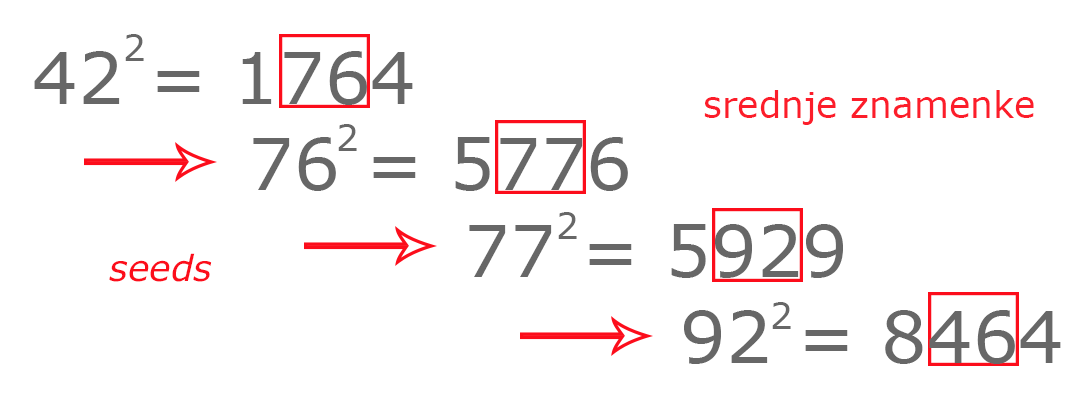
\includegraphics[scale=0.2]{von_neumann.png}
    \caption{Primjer provođenja algoritma}
    \label{fig:von_neumann}
\end{figure}
Pogledajmo također implementaciju ovog algoritma u programskom jeziku \foreign{Python}:

\begin{lstlisting}[language=Python]
seed_number = int(input("Please enter a four digit number:\n[####] "))
number = seed_number
already_seen = set()
counter = 0

while number not in already_seen:
    counter += 1
    already_seen.add(number)
    number = int(str(number * number).zfill(8)[2:6]) 
    print(f"#{counter}: {number}")

print(f"We began with {seed_number}, and"
      f" have repeated ourselves after {counter} steps"
      f" with {number}.")
\end{lstlisting}

\subsection{Linearni posmični generatori}
Pokazat ćemo da su \foreign{xorshift} generator, kreatora \foreign{Marsaglia}e i \foreign{linear-feedback shift register} (u nastavku \foreign{LFSR}) generator, koji je osmislio \foreign{Tausworthe} veoma slični. Preciznije, pokazat ćemo, da uz određene uvjete, \foreign{xorshift} i \foreign{LFSR} generatori mogu generirati isti niz. Najprije definirajmo neke pojmove, koji će nam pomoći pri razumijevanju dokaza.

\begin{napomena}
Definiramo $\poljef$ kao konačno polje s dva elementa $\{0,1\}$. Operacije u polju zapisujemo kao $+$ i $\times$. Ukoliko nam $0$ predstavlja laž, a $1$ istinu, tada su operacije u polju "isključivo ili" (\texttt{xor} ili $\oplus$) te "i" ($\wedge$).
\end{napomena}
\begin{definicija}
Neka je $A \in \poljef^{n\times n}$ matrica reda $n$ nad poljem $\poljef$. \emph{Karakteristični polinom} $\charpol{A}{z}$ matrice $A$ definiramo sa
\begin{equation}
    \charpol{A}{z} = \det(A-zI)\text.
\end{equation}
\end{definicija}
\begin{teorem}[Hamilton--Cayley]\label{tm:HC}
Neka je $A \in \poljef^{n\times n}$ matrica reda $n$ nad poljem $\poljef$. Tada $A$ poništava svoj karakteristični polinom, tj.\
\begin{equation}
    \charpol{A}{A} = 0\text.
\end{equation}
\end{teorem}
\begin{definicija}
\emph{Minimalni polinom} od $A$ je jedinstveni normirani polinom $\minpol{A}{z}$ najmanjeg stupnja takav da je $\minpol{A}{A}=0$ (kojeg $A$ poništava).
\end{definicija}
\begin{napomena}
Očito $\minpol{A}{z}$ dijeli $\charpol{A}{z}$.
\end{napomena}
\begin{definicija}
Neka je $A$ regularna. \emph{Period} matrice A jest najmanji pozitivni cijeli broj $\rho$ takav da je $A^p = I$.
\end{definicija}
\begin{napomena}\label{nap:ired}
Iz teorema~\ref{tm:HC} slijedi da bilo koja pozitivna potencija matrice $A$ može biti prikazana kao linearna kombinacija elemenata skupa $\{I, A, A^2, A^3, \dots, A^{n-1}\}$ te da postoji najviše $2^n -1$ netrivijalnih mogućnosti. Dakle, $\rho \leq 2^n -1$. Maksimalni period $\rho = 2^n -1$ se dobije ako i samo ako je minimalni polinom $\minpol{A}{z}$ ireducibilni polinom stupnja $n$.
\end{napomena}

\begin{definicija}
\emph{LFSR niz} jest niz $(x_j)$ koji zadovoljava linearnu rekurziju 
\begin{equation}\label{eq:recursion}
    \sumk \alpha_k x_{j-k} = 0, \text{ za sve } j \geq d\text,
\end{equation}
gdje su $\alpha_0, \alpha_1, \dots , \alpha_d \in \poljef$ te pretpostavljamo da je $\alpha_0 = 1$. Takva rekurzija definira $x_j$ kao linearnu kombinaciju elemenata $x_{j-1}, \dots, x_{j-d}$. Ukoliko su $x_0, x_1, \dots, x_{d-1}$ dani kao početni uvjeti, tada su svi $x_j$, za $j\geq d$ jedinstveno definirani rekurzijom.
\end{definicija}
Linearna kombinacija $x_j$ može biti samo jedan bit ili cijela riječ. Mi ćemo pretpostaviti da $x_j$ mogu biti skalari ili vektori bilo kakve fiksne veličine. Tada su koeficijenti $\alpha_0, \alpha_1, \dots, \alpha_d$ (\foreign{feedback} koeficijenti) jedinstveno re\-pre\-zen\-ti\-ra\-ni \foreign{LFSR} polinomom povezanosti (\foreign{feedback} polinomom)
\begin{equation}
    P(z) = \sumk \alpha_k z^k\text,
\end{equation}
koji odgovara rekurziji~\eqref{eq:recursion} te je pripadna funkcija izvodnica jednaka $G(z) = \sum_{m=0}^{\infty} x_m z^m$. Ukoliko funkciju izvodnicu promatramo kao for\-mal\-ni red, tada imamo $G(x)= \frac{P_0(z)}{P(z)}$, gdje je $P_0(z)$ polinom stupnja ne većeg od $d-1$, ovisno o početnim uvjetima. Ukoliko je $P(z)$ ireducibilan polinom stupnja $d$ i $P_0(z) \neq 0$, tada je niz $(x_j)$ periodičan s periodom $2^d -1$. Povežimo sada niz generiran \foreign{LFSR} generatorom s nizom generiranim s \foreign{xorshift} generatorom.
Neka je $\beta \in \poljef^{1 \times n}$ netrivijalni vektor čije su komponente u $\poljef$. Vektor $\beta$ možemo promatrati kao \foreign{seed} za \foreign{xorshift} generator. Neka je $T \in \poljef^{n\times n}$ regularna matrica reda $n$ nad poljem $\poljef$. Tada je pseudoslučajni niz $n$-bitnih vektora definiran sa
\begin{equation}\label{eq:xj}
x_j = \beta T^j
\end{equation}
te je generiran koristeći rekurziju $x_j = x_{j-1}T$, za $j \geq 1$, gdje je $x_0 = \beta$. S prikladnim odabirom matrice $T$, dobijemo $32$-bitne i $64$-bitne generatore. \foreign{Marsaglia} je imao ideju uzeti 
\begin{equation}
T = (I + L^a)(I + R^b)(I+L^c)\text,
\end{equation}
gdje su
\begin{gather}
L=\begin{bmatrix}
0 & 0 & \cdots & 0 \\
1 & 0 & \cdots & 0 \\
\vdots & \ddots & \ddots & \vdots \\
0 & \cdots & 1 & 0
\end{bmatrix}
\\[2ex]
R = L^T
\end{gather}
redom lijeve i desne posmične matrice takve da vrijedi
\begin{align}
(v_1v_2 \dots v_{n-1}v_n)L &= (v_2v_3 \dots v_n0)\\
(v_1v_2 \dots v_{n-1}v_n)R &= (0v_1 \dots v_{n-2}v_{n-1})
\end{align}
gdje je $(a,b,c)$ uređena trojka cijelih brojeva.
$T$ je dobro odabran ukoliko je njegov period najveći mogući, tj. $\rho = 2^n -1$. Drugim riječima, $T^{\rho} = I$, a $T^j \neq I$, za $0<j<\rho = 2^n -1$. Iz napomene~\ref{nap:ired} možemo zaključiti da je to istina samo ukoliko je minimalni polinom od $T$ ireducibilni polinom stupnja $n$. Neka je stoga $\minpol{T}{z} = \sum_{k=0}^{d} \alpha_k z^{d-k}$. Možemo pretpostaviti da je $\minpol{T}{z}$ stupnja $d \leq n$ te da je $\alpha_0 = 1$ pa je
\begin{equation}
    \sumk \alpha_k T^{d-k} = 0\text.
\end{equation}
Pomnožimo li slijeva sa $\beta T^{j-d}$, imamo
\begin{equation}
    \sumk \alpha_k \beta T^{j-k} = 0, \text{ za sve } j \geq d\text.
\end{equation}
Kako znamo da je $x_j = \beta T^j$ (jer je $\beta$ \foreign{seed}), slijedi da je
\begin{equation}
    \sumk\alpha_k x_{j-k} = 0, \text{ za sve } j \geq d\text.
\end{equation}
Vidimo da je ovo zapravo linearna rekurzija~\eqref{eq:recursion} koju smo već promatrali. Stoga možemo zaključiti da promatrani niz $(x_j)$ može generirati i \foreign{LFSR} čiji je \foreign{feedback} polinom jednak $\widetilde{P}(z) = \sumk \alpha_k z^k$~\cite{article}. Pokazali smo da \foreign{xorshift} i \foreign{LFSR} generator mogu generirati iste nizove, međutim, ovi generatori ipak se razlikuju. Implementacija \foreign{xorshift}a zahtjeva manje memorije te \texttt{xor} i \texttt{shift} operacija od standardne implementacije \foreign{LFSR} generatora, što ga čini bitno bržim.

\subsection{Usporedba \emph{PRNG} i \emph{TRNG}}
Osim generatora pseudoslučajnih brojeva (\foreign{PRNG}), postoje i generatori "pravih" slučajnih brojeva (\foreign{TRNG}). Takvi generatori izvode slučajnost iz fizičkih fenomena, poput varijacije u pokretima miša ili vrijeme između pritiska dvije tipke na tipkovnici. Atmosferski i termalni šum, elektromagnetski i kvantni fenomeni, kao i radijacija i radioaktivno raspadanje mjereno u kratkim vremenskim intervalima, mogu biti dobri izvori (\foreign{seeds}) prirodne entropije. Generatori "pravih" slučajnih brojeva su, za razliku od generatora pseudoslučajnih brojeva, nedeterministički i aperiodički, ali su i bitno sporiji. Usporedbu svojstava ova dva tipa generatora slučajnih brojeva možete vidjeti u tablici~\ref{tab:razlike}.

\begin{table}[H]
\centering
\caption{Usporedba \emph{PRNG} i \emph{TRNG}}\label{tab:razlike}
\begin{tabular}{|c|c|c|}
\hline
\textbf{Svojstva} & \textbf{Generatori pseudoslučajnih brojeva} & \textbf{Generatori "pravih" brojeva} \\ \hline
učinkovitost      & izvrsno                                     & loše                                 \\ \hline
determinizam      & deterministički                             & nedeterministički                    \\ \hline
periodičnost      & periodički                                  & aperiodički                          \\ \hline
\end{tabular}
\end{table}
Osim po svojstvima, možemo ih usporediti i ovisno o području primjene. Kako je \foreign{TRNG} nedeterministički te je sporiji od \foreign{PRNG}, manje je prikladan za simulacije i modeliranje, gdje se radi s velikim brojem podataka, koje je bi \foreign{PRNG} puno brže izgenerirao. Međutim, u tablici~\ref{tab:primjena} možete vidjeti da \foreign{TRNG} ipak nalazi svoje široko područje primjene.

\begin{table}[H]
\centering
\caption{Područje primjene \textit{PRNG} i \textit{TRNG}}\label{tab:primjena}
\begin{tabular}{|c|c|}
\hline
\textbf{Primjena} & \textbf{Najprikladniji generator} \\ \hline
lutrije           & TRNG                              \\ \hline
igre i kockanje   & TRNG                              \\ \hline
slučajni uzorci   & TRNG                              \\ \hline
sigurnost         & TRNG                              \\ \hline
simulacije        & PRNG                              \\ \hline
\end{tabular}
\end{table}

\section{Primjena generatora slučajnih brojeva}
Već u samom \LaTeX u možemo naići na slučajne brojeve. Postavljanjem izvora na neki broj i koristeći \LaTeX ov generator pseudoslučajnih brojeva, dobili smo sliku~\ref{fig:kruznice} koja prikazuje nepreklapajuće kružnice čija središta imaju slučajnu poziciju unutar zadanog pravokutnika.
\begin{figure}[H]
\centering
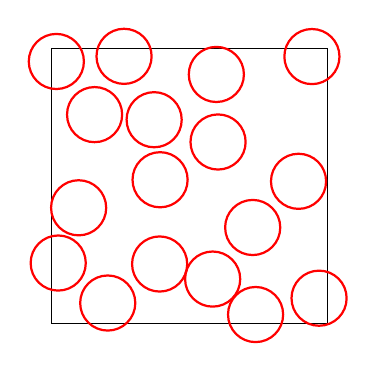
\begin{tikzpicture}[scale=0.7]
\pgfmathsetseed{2}
\fillrandomly{5}{5}{0.5}{300}
\end{tikzpicture}
\caption{Kružnice čija je pozicija slučajna}
\label{fig:kruznice}
\end{figure}
Kao što smo već spomenuli, generatori slučajnih brojeva primjenjuju se u simulacijama. Ukoliko simuliramo prirodne procese, htjeli bismo da oni budu što vjernije prikazani. To se postiže uz pomoć slučajnih brojeva koji su uvelike pridonijeli realističnijim prikazima u području nuklearne fizike i operacijskog istraživanja. U kriptografiji slučajni brojevi igraju izuzetno veliku ulogu. Važnost društvenih mreža i sigurnosti danas je veća nego ikad. Svakom korisniku raznih usluga na internetu važna je privatnost i zaštita osobnih podataka. Stoga je u kriptografiji nužno osigurati neprevidivost brojeva u generiranom nizu. Ulaz u generator mora biti odabran tako da ga je skoro pa nemoguće otkriti nekom metodom pogađanja. Uz to, period generatora mora biti velik, kako bi se postigao velik broj različitih nizova koje je nemoguće pretražiti u konačnom vremenu. Ukoliko je ulaz prikladno odabran te je period dovoljno velik, tada se takav niz može koristiti npr.\ kao tajni ključ za slanje poruka. Generatori slučajnih brojeva koriste se i u numeričkoj analizi. Jednostavan primjer je približno računanje površine kruga. Kockanje, kartanje i računarske igre su možda ipak najpopularniji primjeri primjene generatora slučajnih brojeva. Odatle i potiče naziv poznatog \foreign{Monte Carlo} algoritma koji također koristi slučajne brojeve. 

\section{Zaključak}
U ovom radu upoznali ste se s osnovnim pojmovima vezano uz slučajne brojeve, nizove te generatore slučajnih brojeva. Tema je veoma aktualna te je brojnim znanstvenicima cilj osmisliti što bolji, sigurniji i brži generator slučajnih brojeva. Vidjeli smo da postoje brojni generatori pseudoslučajnih brojeva, a da isto tako postoje brojne ideje za stvaranje novih i boljih generatora "pravih" slučajnih brojeva. Generatori su važni u raznim područjima, od kojih je bitno spomenuti kriptografiju, kockarnice i računalne igre. Rastom tehnologije i interesa ljudi za zaštitu svoje privatnosti, generatori slučajnih brojeva dobivaju na važnosti, stoga će biti zanimljivo vidjeti koja nova prirodna ili fizička pojava bi mogla poslužiti kao izvor raznim generatorima. 


\pagebreak[4]

\printbibliography
\nocite{*}

\end{document}

